\documentclass[11pt]{article}
\usepackage[review]{acl}
\usepackage{times}
\usepackage{latexsym}
\usepackage[T1]{fontenc}
\usepackage[utf8]{inputenc}
\usepackage{microtype}
\usepackage{inconsolata}
\usepackage{graphicx}
\usepackage{booktabs}
\usepackage{array}
\usepackage{amsmath,amssymb}
\usepackage{url}
\usepackage{hyperref}
\hypersetup{hidelinks}
%%%%% NEW MATH DEFINITIONS %%%%%

\usepackage{amsmath,amsfonts,bm}

% Mark sections of captions for referring to divisions of figures
\newcommand{\figleft}{{\em (Left)}}
\newcommand{\figcenter}{{\em (Center)}}
\newcommand{\figright}{{\em (Right)}}
\newcommand{\figtop}{{\em (Top)}}
\newcommand{\figbottom}{{\em (Bottom)}}
\newcommand{\captiona}{{\em (a)}}
\newcommand{\captionb}{{\em (b)}}
\newcommand{\captionc}{{\em (c)}}
\newcommand{\captiond}{{\em (d)}}

% Highlight a newly defined term
\newcommand{\newterm}[1]{{\bf #1}}


% Figure reference, lower-case.
\def\figref#1{figure~\ref{#1}}
% Figure reference, capital. For start of sentence
\def\Figref#1{Figure~\ref{#1}}
\def\twofigref#1#2{figures \ref{#1} and \ref{#2}}
\def\quadfigref#1#2#3#4{figures \ref{#1}, \ref{#2}, \ref{#3} and \ref{#4}}
% Section reference, lower-case.
\def\secref#1{section~\ref{#1}}
% Section reference, capital.
\def\Secref#1{Section~\ref{#1}}
% Reference to two sections.
\def\twosecrefs#1#2{sections \ref{#1} and \ref{#2}}
% Reference to three sections.
\def\secrefs#1#2#3{sections \ref{#1}, \ref{#2} and \ref{#3}}
% Reference to an equation, lower-case.
\def\eqref#1{equation~\ref{#1}}
% Reference to an equation, upper case
\def\Eqref#1{Equation~\ref{#1}}
% A raw reference to an equation---avoid using if possible
\def\plaineqref#1{\ref{#1}}
% Reference to a chapter, lower-case.
\def\chapref#1{chapter~\ref{#1}}
% Reference to an equation, upper case.
\def\Chapref#1{Chapter~\ref{#1}}
% Reference to a range of chapters
\def\rangechapref#1#2{chapters\ref{#1}--\ref{#2}}
% Reference to an algorithm, lower-case.
\def\algref#1{algorithm~\ref{#1}}
% Reference to an algorithm, upper case.
\def\Algref#1{Algorithm~\ref{#1}}
\def\twoalgref#1#2{algorithms \ref{#1} and \ref{#2}}
\def\Twoalgref#1#2{Algorithms \ref{#1} and \ref{#2}}
% Reference to a part, lower case
\def\partref#1{part~\ref{#1}}
% Reference to a part, upper case
\def\Partref#1{Part~\ref{#1}}
\def\twopartref#1#2{parts \ref{#1} and \ref{#2}}

\def\ceil#1{\lceil #1 \rceil}
\def\floor#1{\lfloor #1 \rfloor}
\def\1{\bm{1}}
\newcommand{\train}{\mathcal{D}}
\newcommand{\valid}{\mathcal{D_{\mathrm{valid}}}}
\newcommand{\test}{\mathcal{D_{\mathrm{test}}}}

\def\eps{{\epsilon}}


% Random variables
\def\reta{{\textnormal{$\eta$}}}
\def\ra{{\textnormal{a}}}
\def\rb{{\textnormal{b}}}
\def\rc{{\textnormal{c}}}
\def\rd{{\textnormal{d}}}
\def\re{{\textnormal{e}}}
\def\rf{{\textnormal{f}}}
\def\rg{{\textnormal{g}}}
\def\rh{{\textnormal{h}}}
\def\ri{{\textnormal{i}}}
\def\rj{{\textnormal{j}}}
\def\rk{{\textnormal{k}}}
\def\rl{{\textnormal{l}}}
% rm is already a command, just don't name any random variables m
\def\rn{{\textnormal{n}}}
\def\ro{{\textnormal{o}}}
\def\rp{{\textnormal{p}}}
\def\rq{{\textnormal{q}}}
\def\rr{{\textnormal{r}}}
\def\rs{{\textnormal{s}}}
\def\rt{{\textnormal{t}}}
\def\ru{{\textnormal{u}}}
\def\rv{{\textnormal{v}}}
\def\rw{{\textnormal{w}}}
\def\rx{{\textnormal{x}}}
\def\ry{{\textnormal{y}}}
\def\rz{{\textnormal{z}}}

% Random vectors
\def\rvepsilon{{\mathbf{\epsilon}}}
\def\rvtheta{{\mathbf{\theta}}}
\def\rva{{\mathbf{a}}}
\def\rvb{{\mathbf{b}}}
\def\rvc{{\mathbf{c}}}
\def\rvd{{\mathbf{d}}}
\def\rve{{\mathbf{e}}}
\def\rvf{{\mathbf{f}}}
\def\rvg{{\mathbf{g}}}
\def\rvh{{\mathbf{h}}}
\def\rvu{{\mathbf{i}}}
\def\rvj{{\mathbf{j}}}
\def\rvk{{\mathbf{k}}}
\def\rvl{{\mathbf{l}}}
\def\rvm{{\mathbf{m}}}
\def\rvn{{\mathbf{n}}}
\def\rvo{{\mathbf{o}}}
\def\rvp{{\mathbf{p}}}
\def\rvq{{\mathbf{q}}}
\def\rvr{{\mathbf{r}}}
\def\rvs{{\mathbf{s}}}
\def\rvt{{\mathbf{t}}}
\def\rvu{{\mathbf{u}}}
\def\rvv{{\mathbf{v}}}
\def\rvw{{\mathbf{w}}}
\def\rvx{{\mathbf{x}}}
\def\rvy{{\mathbf{y}}}
\def\rvz{{\mathbf{z}}}

% Elements of random vectors
\def\erva{{\textnormal{a}}}
\def\ervb{{\textnormal{b}}}
\def\ervc{{\textnormal{c}}}
\def\ervd{{\textnormal{d}}}
\def\erve{{\textnormal{e}}}
\def\ervf{{\textnormal{f}}}
\def\ervg{{\textnormal{g}}}
\def\ervh{{\textnormal{h}}}
\def\ervi{{\textnormal{i}}}
\def\ervj{{\textnormal{j}}}
\def\ervk{{\textnormal{k}}}
\def\ervl{{\textnormal{l}}}
\def\ervm{{\textnormal{m}}}
\def\ervn{{\textnormal{n}}}
\def\ervo{{\textnormal{o}}}
\def\ervp{{\textnormal{p}}}
\def\ervq{{\textnormal{q}}}
\def\ervr{{\textnormal{r}}}
\def\ervs{{\textnormal{s}}}
\def\ervt{{\textnormal{t}}}
\def\ervu{{\textnormal{u}}}
\def\ervv{{\textnormal{v}}}
\def\ervw{{\textnormal{w}}}
\def\ervx{{\textnormal{x}}}
\def\ervy{{\textnormal{y}}}
\def\ervz{{\textnormal{z}}}

% Random matrices
\def\rmA{{\mathbf{A}}}
\def\rmB{{\mathbf{B}}}
\def\rmC{{\mathbf{C}}}
\def\rmD{{\mathbf{D}}}
\def\rmE{{\mathbf{E}}}
\def\rmF{{\mathbf{F}}}
\def\rmG{{\mathbf{G}}}
\def\rmH{{\mathbf{H}}}
\def\rmI{{\mathbf{I}}}
\def\rmJ{{\mathbf{J}}}
\def\rmK{{\mathbf{K}}}
\def\rmL{{\mathbf{L}}}
\def\rmM{{\mathbf{M}}}
\def\rmN{{\mathbf{N}}}
\def\rmO{{\mathbf{O}}}
\def\rmP{{\mathbf{P}}}
\def\rmQ{{\mathbf{Q}}}
\def\rmR{{\mathbf{R}}}
\def\rmS{{\mathbf{S}}}
\def\rmT{{\mathbf{T}}}
\def\rmU{{\mathbf{U}}}
\def\rmV{{\mathbf{V}}}
\def\rmW{{\mathbf{W}}}
\def\rmX{{\mathbf{X}}}
\def\rmY{{\mathbf{Y}}}
\def\rmZ{{\mathbf{Z}}}

% Elements of random matrices
\def\ermA{{\textnormal{A}}}
\def\ermB{{\textnormal{B}}}
\def\ermC{{\textnormal{C}}}
\def\ermD{{\textnormal{D}}}
\def\ermE{{\textnormal{E}}}
\def\ermF{{\textnormal{F}}}
\def\ermG{{\textnormal{G}}}
\def\ermH{{\textnormal{H}}}
\def\ermI{{\textnormal{I}}}
\def\ermJ{{\textnormal{J}}}
\def\ermK{{\textnormal{K}}}
\def\ermL{{\textnormal{L}}}
\def\ermM{{\textnormal{M}}}
\def\ermN{{\textnormal{N}}}
\def\ermO{{\textnormal{O}}}
\def\ermP{{\textnormal{P}}}
\def\ermQ{{\textnormal{Q}}}
\def\ermR{{\textnormal{R}}}
\def\ermS{{\textnormal{S}}}
\def\ermT{{\textnormal{T}}}
\def\ermU{{\textnormal{U}}}
\def\ermV{{\textnormal{V}}}
\def\ermW{{\textnormal{W}}}
\def\ermX{{\textnormal{X}}}
\def\ermY{{\textnormal{Y}}}
\def\ermZ{{\textnormal{Z}}}

% Vectors
\def\vzero{{\bm{0}}}
\def\vone{{\bm{1}}}
\def\vmu{{\bm{\mu}}}
\def\vtheta{{\bm{\theta}}}
\def\va{{\bm{a}}}
\def\vb{{\bm{b}}}
\def\vc{{\bm{c}}}
\def\vd{{\bm{d}}}
\def\ve{{\bm{e}}}
\def\vf{{\bm{f}}}
\def\vg{{\bm{g}}}
\def\vh{{\bm{h}}}
\def\vi{{\bm{i}}}
\def\vj{{\bm{j}}}
\def\vk{{\bm{k}}}
\def\vl{{\bm{l}}}
\def\vm{{\bm{m}}}
\def\vn{{\bm{n}}}
\def\vo{{\bm{o}}}
\def\vp{{\bm{p}}}
\def\vq{{\bm{q}}}
\def\vr{{\bm{r}}}
\def\vs{{\bm{s}}}
\def\vt{{\bm{t}}}
\def\vu{{\bm{u}}}
\def\vv{{\bm{v}}}
\def\vw{{\bm{w}}}
\def\vx{{\bm{x}}}
\def\vy{{\bm{y}}}
\def\vz{{\bm{z}}}

% Elements of vectors
\def\evalpha{{\alpha}}
\def\evbeta{{\beta}}
\def\evepsilon{{\epsilon}}
\def\evlambda{{\lambda}}
\def\evomega{{\omega}}
\def\evmu{{\mu}}
\def\evpsi{{\psi}}
\def\evsigma{{\sigma}}
\def\evtheta{{\theta}}
\def\eva{{a}}
\def\evb{{b}}
\def\evc{{c}}
\def\evd{{d}}
\def\eve{{e}}
\def\evf{{f}}
\def\evg{{g}}
\def\evh{{h}}
\def\evi{{i}}
\def\evj{{j}}
\def\evk{{k}}
\def\evl{{l}}
\def\evm{{m}}
\def\evn{{n}}
\def\evo{{o}}
\def\evp{{p}}
\def\evq{{q}}
\def\evr{{r}}
\def\evs{{s}}
\def\evt{{t}}
\def\evu{{u}}
\def\evv{{v}}
\def\evw{{w}}
\def\evx{{x}}
\def\evy{{y}}
\def\evz{{z}}

% Matrix
\def\mA{{\bm{A}}}
\def\mB{{\bm{B}}}
\def\mC{{\bm{C}}}
\def\mD{{\bm{D}}}
\def\mE{{\bm{E}}}
\def\mF{{\bm{F}}}
\def\mG{{\bm{G}}}
\def\mH{{\bm{H}}}
\def\mI{{\bm{I}}}
\def\mJ{{\bm{J}}}
\def\mK{{\bm{K}}}
\def\mL{{\bm{L}}}
\def\mM{{\bm{M}}}
\def\mN{{\bm{N}}}
\def\mO{{\bm{O}}}
\def\mP{{\bm{P}}}
\def\mQ{{\bm{Q}}}
\def\mR{{\bm{R}}}
\def\mS{{\bm{S}}}
\def\mT{{\bm{T}}}
\def\mU{{\bm{U}}}
\def\mV{{\bm{V}}}
\def\mW{{\bm{W}}}
\def\mX{{\bm{X}}}
\def\mY{{\bm{Y}}}
\def\mZ{{\bm{Z}}}
\def\mBeta{{\bm{\beta}}}
\def\mPhi{{\bm{\Phi}}}
\def\mLambda{{\bm{\Lambda}}}
\def\mSigma{{\bm{\Sigma}}}

% Tensor
\DeclareMathAlphabet{\mathsfit}{\encodingdefault}{\sfdefault}{m}{sl}
\SetMathAlphabet{\mathsfit}{bold}{\encodingdefault}{\sfdefault}{bx}{n}
\newcommand{\tens}[1]{\bm{\mathsfit{#1}}}
\def\tA{{\tens{A}}}
\def\tB{{\tens{B}}}
\def\tC{{\tens{C}}}
\def\tD{{\tens{D}}}
\def\tE{{\tens{E}}}
\def\tF{{\tens{F}}}
\def\tG{{\tens{G}}}
\def\tH{{\tens{H}}}
\def\tI{{\tens{I}}}
\def\tJ{{\tens{J}}}
\def\tK{{\tens{K}}}
\def\tL{{\tens{L}}}
\def\tM{{\tens{M}}}
\def\tN{{\tens{N}}}
\def\tO{{\tens{O}}}
\def\tP{{\tens{P}}}
\def\tQ{{\tens{Q}}}
\def\tR{{\tens{R}}}
\def\tS{{\tens{S}}}
\def\tT{{\tens{T}}}
\def\tU{{\tens{U}}}
\def\tV{{\tens{V}}}
\def\tW{{\tens{W}}}
\def\tX{{\tens{X}}}
\def\tY{{\tens{Y}}}
\def\tZ{{\tens{Z}}}


% Graph
\def\gA{{\mathcal{A}}}
\def\gB{{\mathcal{B}}}
\def\gC{{\mathcal{C}}}
\def\gD{{\mathcal{D}}}
\def\gE{{\mathcal{E}}}
\def\gF{{\mathcal{F}}}
\def\gG{{\mathcal{G}}}
\def\gH{{\mathcal{H}}}
\def\gI{{\mathcal{I}}}
\def\gJ{{\mathcal{J}}}
\def\gK{{\mathcal{K}}}
\def\gL{{\mathcal{L}}}
\def\gM{{\mathcal{M}}}
\def\gN{{\mathcal{N}}}
\def\gO{{\mathcal{O}}}
\def\gP{{\mathcal{P}}}
\def\gQ{{\mathcal{Q}}}
\def\gR{{\mathcal{R}}}
\def\gS{{\mathcal{S}}}
\def\gT{{\mathcal{T}}}
\def\gU{{\mathcal{U}}}
\def\gV{{\mathcal{V}}}
\def\gW{{\mathcal{W}}}
\def\gX{{\mathcal{X}}}
\def\gY{{\mathcal{Y}}}
\def\gZ{{\mathcal{Z}}}

% Sets
\def\sA{{\mathbb{A}}}
\def\sB{{\mathbb{B}}}
\def\sC{{\mathbb{C}}}
\def\sD{{\mathbb{D}}}
% Don't use a set called E, because this would be the same as our symbol
% for expectation.
\def\sF{{\mathbb{F}}}
\def\sG{{\mathbb{G}}}
\def\sH{{\mathbb{H}}}
\def\sI{{\mathbb{I}}}
\def\sJ{{\mathbb{J}}}
\def\sK{{\mathbb{K}}}
\def\sL{{\mathbb{L}}}
\def\sM{{\mathbb{M}}}
\def\sN{{\mathbb{N}}}
\def\sO{{\mathbb{O}}}
\def\sP{{\mathbb{P}}}
\def\sQ{{\mathbb{Q}}}
\def\sR{{\mathbb{R}}}
\def\sS{{\mathbb{S}}}
\def\sT{{\mathbb{T}}}
\def\sU{{\mathbb{U}}}
\def\sV{{\mathbb{V}}}
\def\sW{{\mathbb{W}}}
\def\sX{{\mathbb{X}}}
\def\sY{{\mathbb{Y}}}
\def\sZ{{\mathbb{Z}}}

% Entries of a matrix
\def\emLambda{{\Lambda}}
\def\emA{{A}}
\def\emB{{B}}
\def\emC{{C}}
\def\emD{{D}}
\def\emE{{E}}
\def\emF{{F}}
\def\emG{{G}}
\def\emH{{H}}
\def\emI{{I}}
\def\emJ{{J}}
\def\emK{{K}}
\def\emL{{L}}
\def\emM{{M}}
\def\emN{{N}}
\def\emO{{O}}
\def\emP{{P}}
\def\emQ{{Q}}
\def\emR{{R}}
\def\emS{{S}}
\def\emT{{T}}
\def\emU{{U}}
\def\emV{{V}}
\def\emW{{W}}
\def\emX{{X}}
\def\emY{{Y}}
\def\emZ{{Z}}
\def\emSigma{{\Sigma}}

% entries of a tensor
% Same font as tensor, without \bm wrapper
\newcommand{\etens}[1]{\mathsfit{#1}}
\def\etLambda{{\etens{\Lambda}}}
\def\etA{{\etens{A}}}
\def\etB{{\etens{B}}}
\def\etC{{\etens{C}}}
\def\etD{{\etens{D}}}
\def\etE{{\etens{E}}}
\def\etF{{\etens{F}}}
\def\etG{{\etens{G}}}
\def\etH{{\etens{H}}}
\def\etI{{\etens{I}}}
\def\etJ{{\etens{J}}}
\def\etK{{\etens{K}}}
\def\etL{{\etens{L}}}
\def\etM{{\etens{M}}}
\def\etN{{\etens{N}}}
\def\etO{{\etens{O}}}
\def\etP{{\etens{P}}}
\def\etQ{{\etens{Q}}}
\def\etR{{\etens{R}}}
\def\etS{{\etens{S}}}
\def\etT{{\etens{T}}}
\def\etU{{\etens{U}}}
\def\etV{{\etens{V}}}
\def\etW{{\etens{W}}}
\def\etX{{\etens{X}}}
\def\etY{{\etens{Y}}}
\def\etZ{{\etens{Z}}}

% The true underlying data generating distribution
\newcommand{\pdata}{p_{\rm{data}}}
% The empirical distribution defined by the training set
\newcommand{\ptrain}{\hat{p}_{\rm{data}}}
\newcommand{\Ptrain}{\hat{P}_{\rm{data}}}
% The model distribution
\newcommand{\pmodel}{p_{\rm{model}}}
\newcommand{\Pmodel}{P_{\rm{model}}}
\newcommand{\ptildemodel}{\tilde{p}_{\rm{model}}}
% Stochastic autoencoder distributions
\newcommand{\pencode}{p_{\rm{encoder}}}
\newcommand{\pdecode}{p_{\rm{decoder}}}
\newcommand{\precons}{p_{\rm{reconstruct}}}

\newcommand{\laplace}{\mathrm{Laplace}} % Laplace distribution

\newcommand{\E}{\mathbb{E}}
\newcommand{\Ls}{\mathcal{L}}
\newcommand{\R}{\mathbb{R}}
\newcommand{\emp}{\tilde{p}}
\newcommand{\lr}{\alpha}
\newcommand{\reg}{\lambda}
\newcommand{\rect}{\mathrm{rectifier}}
\newcommand{\softmax}{\mathrm{softmax}}
\newcommand{\sigmoid}{\sigma}
\newcommand{\softplus}{\zeta}
\newcommand{\KL}{D_{\mathrm{KL}}}
\newcommand{\Var}{\mathrm{Var}}
\newcommand{\standarderror}{\mathrm{SE}}
\newcommand{\Cov}{\mathrm{Cov}}
% Wolfram Mathworld says $L^2$ is for function spaces and $\ell^2$ is for vectors
% But then they seem to use $L^2$ for vectors throughout the site, and so does
% wikipedia.
\newcommand{\normlzero}{L^0}
\newcommand{\normlone}{L^1}
\newcommand{\normltwo}{L^2}
\newcommand{\normlp}{L^p}
\newcommand{\normmax}{L^\infty}

\newcommand{\parents}{Pa} % See usage in notation.tex. Chosen to match Daphne's book.

\DeclareMathOperator*{\argmax}{arg\,max}
\DeclareMathOperator*{\argmin}{arg\,min}

\DeclareMathOperator{\sign}{sign}
\DeclareMathOperator{\Tr}{Tr}
\let\ab\allowbreak


\title{Before Candidate Selection in Test-Time LLM Agents: A Scope-Limited Audit of Exposure, Score Interventions, and Realized Candidate Support}
\author{Anonymous ACL Submission}

\begin{document}
\maketitle

\begin{abstract}
Test-time LLM agents retain natural-language state, score intermediate responses, and revise their outputs while solving tasks. Before adding a candidate selector or a privacy mechanism, one should check three preconditions: whether protected content enters persistent state, whether changing the score has downstream consequences, and whether the generator exposes executable alternatives worth selecting. We apply this audit order to one configuration of a released multi-agent runtime, TacoMAS with a fixed three-agent topology and structural edits disabled, on the PlanCraft benchmark. In a three-arm canary study with 120 instances per arm (360 runs), no exact or five-token partial canary was recovered from post-input persistent state under our canary family, injection route, observer, and five-round horizon (evolve-arm one-sided 95\% upper bound 2.5\%). Removing the fast-round length term, which carries 85\% of the heuristic score weight, sharply lowers recorded scores for DeepSeek and Qwen, but exactness effects in the primary cohorts are heterogeneous and inconclusive. In four frozen cohorts, 43 of 46 failed runs contain no parser-accepted executable candidate in the recorded pool, so selectors restricted to that pool could have gained only 0--8.3 percentage points. Adding four independent stochastic restarts raises the offline executable oracle from 0.60 to 0.80 at roughly three times the token cost. These results scope where selection and privacy mechanisms could matter in this runtime; they do not provide end-to-end privacy or a general prevalence estimate.
\end{abstract}

\section{Introduction}

Language-model agents increasingly adapt while solving a task. They revise role prompts, summarize natural-language memories, assign contribution scores, and change workflows or communication structure. TacoMAS exemplifies this design: a fast loop produces and evaluates agent outputs, while a slower controller can update feedback and topology \citep{xu2026tacomas}. Such systems invite a natural privacy proposal. If an input can enter persistent state, privatize the scores or decisions that update that state.

This proposal joins two questions that need not have the same answer. A mechanism can provide a valid event-level DP guarantee for a bounded score while protecting a decision with negligible task value. Conversely, a useful candidate selector says nothing about whether natural-language memories and messages are private. Before measuring a privacy--utility frontier, three empirical premises must hold:
\begin{enumerate}
    \setlength{\itemsep}{1pt}
    \item protected information measurably enters post-input persistent state
    \item changing the score to be privatized has a detectable consequence for executable utility
    \item the realized candidate pool contains a better output worth selecting.
\end{enumerate}
Architecture diagrams do not establish any of them. A model may fail to retain a tested secret over a short horizon. A ``contribution'' score may mostly reward verbose text. A perfect selector cannot recover a candidate the generator never produced.

We organize these checks into a scope-limited audit and apply it to one configuration of TacoMAS on PlanCraft, a tool-using crafting benchmark with deterministic action-list evaluation \citep{dagan2025plancraft}. Structural birth/death and edge edits are disabled in every study, so all runs share a fixed three-agent topology; the results describe this fixed-topology slice of the runtime, not topology evolution. In this configuration we did not detect the motivating post-input canary channel, removing the dominant score term did not reliably change exactness, and most failed runs contained no parser-accepted executable candidate that a selector restricted to the recorded pool could recover.

These checks point to generation support rather than selection as the binding constraint in this configuration. Adding independent restarts expands the recorded support and raises the offline oracle by 20 points, at triple the token cost. Table~\ref{tab:roadmap} maps each premise to its verdict, and Appendix~\ref{app:procedure} states the audit as a procedure with the frozen stop rules used here.

\begin{table}[t]
\caption{Audit roadmap: each premise and its verdict in the audited configuration.}
\label{tab:roadmap}
\centering
\small
\setlength{\tabcolsep}{3pt}
\begin{tabular}{>{\raggedright\arraybackslash}p{0.33\columnwidth}>{\raggedright\arraybackslash}p{0.61\columnwidth}}
\toprule
Premise (section) & Verdict \\
\midrule
Post-input exposure (\S\ref{sec:res-audit}) & Not detected; 0/120 per arm, upper bound 2.5\% \\
Score consequence (\S\ref{sec:res-audit}) & Score shifts; primary exactness effects heterogeneous and inconclusive \\
Candidate support (\S\ref{sec:res-headroom}) & 43/46 failures lack a parser-accepted executable candidate; 0--8.3 points of headroom \\
Support expansion (\S\ref{sec:res-expand}) & Offline oracle $0.60\to0.80$ at $3\times$ tokens \\
\bottomrule
\end{tabular}
\end{table}

Our contribution is the audit order and its application, not a new algorithm: the hindsight oracle gap, term ablation, and canary matching are standard tools. Specifically, we contribute:
\begin{itemize}
    \setlength{\itemsep}{1pt}
    \item a scope-limited audit order that checks exposure, score consequences, and realized executable support before any privacy budget is spent, with explicit stop rules
    \item an executable audit of a fixed-topology TacoMAS--PlanCraft configuration in which the realized-pool oracle gap bounds every selector restricted to the recorded candidates
    \item prospective evidence that additional independent restarts expand recorded support, with a retrospective slot-matched decomposition
    \item a scoped diagnostic on two selected hard failures showing task-level response collapse under both repair-conditioned and public-only prompts.
\end{itemize}
We do not present a new end-to-end private agent or a general leakage estimate.

\section{Auditing Selection Preconditions}

\subsection{Persistent exposure after the input disappears}

At round $t$, agent $v$ has persistent text-bearing state
\[
s_{v,t}=(\phi_{v,t},m_{v,t},f_{v,t},o_{v,t},q_{v,t}),
\]
covering policy text, memory, feedback, stored outputs, and score history. A canary placed in the round-one query trivially occurs in that query and may be echoed immediately. We therefore define leakage operationally as exact or frozen five-token partial recovery from persistent state at rounds 3 or 5, after the direct-input checkpoint.

The audit uses three five-round arms: evolution with a canary, a depth-matched reset that restores initial state after each round, and evolution without a canary. The reset control distinguishes persistence created by state evolution from ordinary processing of a repeated task. We snapshot every declared text channel, store only match metadata in research artifacts, and separately verify the extractor by deterministic channel injection and a live memory-write positive control. Appendix~\ref{app:threat} states the threat model for this audit and for the selector calculation.

\subsection{Score consequences before privacy calibration}

The released non-slow-round score is
\[
\begin{aligned}
c(y,e)={}&0.85\min\{1,|y|/800\}\\
&+0.15\mathbf 1\{e=\mathrm{success}\},
\end{aligned}
\]
where $|y|$ is the response length and $e$ the environment outcome. Length can therefore move the score much more than environment success. To measure consequences rather than correlation, we compare, on the same tasks, the released score with a length-term-removal arm in which the 0.85 length weight is set to zero (``length-zero'' in our artifacts), holding prompts, topology, rounds, feedback opportunities, and structural masks fixed. The design is paired and prospective: both arms run on every task under the same frozen schedule. References are withheld until generation finishes and reference exactness is computed offline, so an evaluator cannot leak the answer into stopping, retention, or feedback.

The runtime authors clarify that this formula is a low-cost heuristic for fast rounds without a slow update, intended as a coarse proxy for analytical effort. During a scheduled slow update, a separately configured Judge LLM produces an independent score; the Meta-LLM receives it together with historical heuristic and judge scores when making topology, edge, feedback, and workflow decisions. In the 60 initial canary-study runs, 705 of 900 recorded contribution scores came from the heuristic and 195 from slow-update judging (Appendix~\ref{app:scoreconsequence}). Zeroing the length term changes every downstream use of the heuristic, including retention, the score history passed to the Meta-LLM, and feedback, and call and token counts differ by arm. Its estimand is therefore the system-level consequence of replacing the fast-round heuristic, not the effect of verbosity alone. A null utility effect would not show that the score is invalid: the controller may ignore it, other signals may dominate, or the cohorts may be underpowered.

For a paired score intervention $Z$ and a final-answer endpoint $V$, define its arm-level consequence as
\[
\widehat\delta_V^{\mathrm{abl}}=
\widehat{\mathbb E}[V\mid Z=1]-\widehat{\mathbb E}[V\mid Z=0].
\]
Table~\ref{tab:audit} uses reference exactness for $V$; executable validity gives identical paired differences in both non-degenerate cohorts (Appendix~\ref{app:scoreconsequence}). This arm-level diagnostic is not a parameter of a candidate selector. For two candidates with utility-score gap $g_U^{\mathrm{sel}}=u(c^+)-u(c^-)$ and candidate-score sensitivity $\Delta_u$, define the separate local selector ratio $\rho_U^{\mathrm{sel}}=g_U^{\mathrm{sel}}/\Delta_u$. Under candidate-score replacement adjacency, a neighboring input changes one candidate's score by at most $\Delta_u$ and leaves the other scores and the candidate set fixed. Such changes are monotone, so sampling candidate $j$ with probability proportional to $\exp(\varepsilon u_j/\Delta_u)$ is $\varepsilon$-DP \citep{mcsherry2007mechanism}; Appendix~\ref{app:selector} gives the proof. Under the general calibration $\exp(\varepsilon u_j/2\Delta_u)$, every budget reported below doubles. With the other $k-1$ candidates tied at the lower utility, the preferred-candidate probability is
\[
\frac{1}{1+(k-1)e^{-\varepsilon\rho_U^{\mathrm{sel}}}}.
\]
If an intervention changes scores but not utility, increasing $\varepsilon$ cannot make the targeted signal useful.

\subsection{Candidate-pool headroom}

Let $f_i$ be run $i$'s synthesized final answer and let $\mathcal C_i$ contain $f_i$ plus all persisted round-agent candidates. For executable utility $U$, define
\[
H_i=\max_{c\in\mathcal C_i}U(c)-U(f_i).
\]
$H_i$ is the hindsight realized-pool oracle gap. It bounds every selector, private or not, whose output must belong to $\mathcal C_i$; it does not constrain regeneration, repair, or new tool interaction, which change $\mathcal C_i$. Including $f_i$ was an outcome-aware amendment, but no eligible run had a valid final answer without a valid round candidate (0/65), so the round-candidate-only oracle gives identical values.

$U$ is executable validity. We parse candidate text into canonical crafting plans and execute them without reference answers; slots the parser rejects count as non-executable, so every headroom claim is conditional on this parser and executor. Reference exactness is computed offline for secondary checks. Appendix~\ref{app:metrics} defines each metric and where it is used.

\subsection{Inference and experimental sequence}

Paired binary effects use task-level risk differences, paired task bootstraps, and exact discordant-pair tests when positive and negative differences are both possible. When a small-sample bootstrap is degenerate, we flag it and give an exact bound. Nested pools satisfy $C_1\subset C_5$, so their support and oracle differences cannot be negative; we report task-bootstrap intervals and one-sided lower bounds, not sign-test $p$-values. Provider calls, rounds, candidate slots, and repeated repairs are never treated as independent task units.

The experiments proceed in a fixed order. We first audit canary exposure and score signals with DeepSeek V4 Flash, then complete a frozen 120-instance replication of the canary audit. We repeat the length-term removal on a non-degenerate DeepSeek cohort and an untouched Qwen3.7-Max cohort. A zero-call oracle audit measures fixed-pool headroom, and a prospective Qwen study expands candidate support with independent restarts. Protocols were frozen as internal JSON records before execution; they are not externally timestamped registrations. An appendix endpoint-status table separates quantities frozen before provider execution from later secondary analyses; no post-outcome qualification changes a recorded run or primary endpoint.

\section{Results}

\subsection{Leakage diagnostic and score consequences}
\label{sec:res-audit}

All 60 cells in the initial 20-instance canary study complete five rounds, with no exact or five-token partial canary in post-input persistent state. We then completed the frozen 120-instance replication (120 runs per arm, 360 runs): all 360 cells reached five rounds, and exposure was 0/120 in the evolve and depth-matched-reset arms; the no-canary arm also had 0/120 false positives. The evolve-arm one-sided 95\% upper confidence bound is 2.5\%. Exposure was zero in each of the three 40-instance strata, and the paired evolve-minus-reset risk difference is 0 with exact two-sided McNemar $p=1$. The extractor recovers 7/7 deterministic channel injections and a live canary written into memory at round 2; these controls show that it detects canaries placed in each declared channel, not that a round-one canary must reach those channels. State is active rather than inert: 617/720 comparable agent transitions change in the initial audit, all 168 recorded slow-feedback fields are nonempty, and retention fires in 60/300 rounds. The replication is a complete failed-to-detect result for this model, horizon, topology, canary family, and observer; it does not establish a privacy guarantee (Figure~\ref{fig:audit}a).

\begin{table*}[t]
\caption{Primary audit diagnostics. $n$ counts runs per arm (canary rows) or task pairs (ablation rows). Exposure is post-input; upper bounds are one-sided 95\%. Ablations report length-removed minus released-score reference exactness; non-degenerate cohorts passed a frozen 30--70\% baseline gate that was blind to the length contrast. $^\dagger$Degenerate bootstrap (0/10 discordant pairs); the exact bound is $|\mathrm{RD}|\le0.31$. The 42-pair synthesis is secondary and outcome-aware. The retention row reports executor-based minus text-heuristic executable validity.}
\label{tab:audit}
\centering
\small
\begin{tabular}{lccc}
\toprule
Study & $n$ & Primary observation & 95\% interval \\
\midrule
Canary: initial evolve & 20 & exact/partial $0/20$ & upper bound 0.139 \\
Canary: initial reset & 20 & exact/partial $0/20$ & upper bound 0.139 \\
Canary: replication evolve & 120 & exact/partial $0/120$ & upper bound 0.025 \\
Canary: replication reset & 120 & exact/partial $0/120$ & upper bound 0.025 \\
No-canary replication & 120 & false positives $0/120$ & upper bound 0.025 \\
DeepSeek initial removal & 10 pairs & ref.\ exactness $0.000$ & $[0,0]^\dagger$ \\
DeepSeek non-degenerate removal & 12 pairs & ref.\ exactness $+0.167$ & $[0,0.417]$ \\
Qwen non-degenerate removal & 20 pairs & ref.\ exactness $-0.050$ & $[-0.250,0.150]$ \\
Secondary synthesis & 42 pairs & ref.\ exactness $+0.024$ & $[-0.095,0.143]$ \\
Execution-aware retention & 20 pairs & executable $+0.050$ & $[0,0.150]$ \\
\bottomrule
\end{tabular}
\end{table*}

\begin{figure*}[t]
\centering
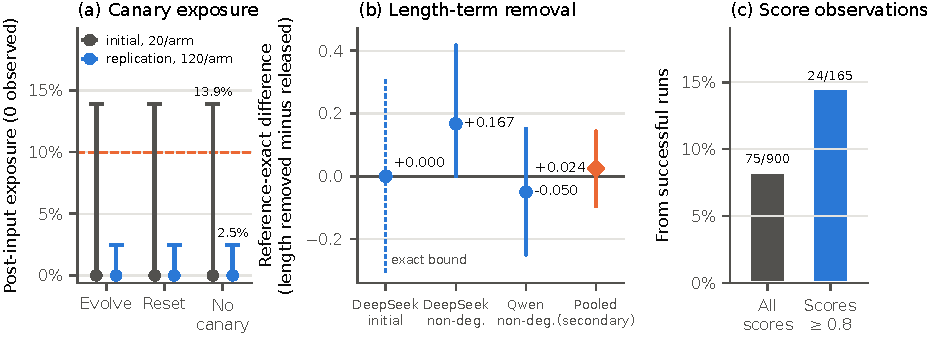
\includegraphics[width=\textwidth]{figures/evolution-audit-main-results.pdf}
\caption{Audit results. (a) No post-input exposure in either study; the replication has 120 runs per arm (360 runs). Whiskers are run-level one-sided 95\% upper bounds; the dashed line is the frozen 10\% gate. (b) Length-removed minus released-score reference exactness with 95\% task-bootstrap intervals; the dashed whisker is the exact bound for the degenerate DeepSeek initial interval, and the pooled synthesis is secondary and outcome-aware. (c) Agent-round score observations in the 60 initial runs (15 per run) that come from the five successful runs: 24 of 165 scores of at least 0.8 versus 75 of 900 overall. Observations are clustered within runs, so this is descriptive, not calibration evidence.}
\label{fig:audit}
\end{figure*}

The score audit separates score movement from task movement. Most scores of at least 0.8 occur in failed runs because failures dominate the cohort; relative to the base rate they are only mildly enriched among successes (Figure~\ref{fig:audit}c), and the run-level AUC of the maximum score is 0.755 (Appendix~\ref{app:bootstrap}). We do not treat these counts as calibration evidence: only five runs are exact, from three task instances.

The paired interventions show that the score responds while exactness does not reliably follow. The two later cohorts are non-degenerate: each ran only after an eight-task gate, blind to the length contrast, placed baseline exactness inside a frozen 30--70\% window. Removing the length term sharply reduces mean contribution score in every study: from 0.429 to 0.069 in the initial DeepSeek pairs, by $-0.308$ $[-0.381,-0.230]$ in the non-degenerate DeepSeek replication, and by $-0.117$ $[-0.150,-0.084]$ in Qwen, eliminating every score of at least 0.8 in the paired cohorts. Exactness effects in the primary cohorts are heterogeneous and inconclusive (Table~\ref{tab:audit}; Figure~\ref{fig:audit}b): zero in the initial pairs, whose bootstrap interval is degenerate (exact bound $\pm0.31$), and $+0.167$ and $-0.050$ in the two non-degenerate cohorts. The DeepSeek $+0.167$ estimate is also within nuisance variation: the three arms of that replication that share the released score span 5/12 to 7/12 exact, the same two-task spread. A secondary, outcome-aware synthesis of all 42 pairs gives $+0.024$ $[-0.095,0.143]$. We therefore claim only that removing the fast-round length term changes recorded scores without a reliably detectable change in measured exactness, not that the score is invalid.

Replacing the heuristic outright does not rescue utility either. Inserting a reference-free executor into historical-answer retention gave 1/8 versus 0/8 executable finals in a development pilot and 1/20 versus 0/20 in a separately frozen validation ($+0.05$ $[0,0.15]$, one-sided exact $p=0.5$), failing the frozen confirmation rule (Appendix~\ref{app:retention}). The text-heuristic arm of that validation is the retention control in Table~\ref{tab:headroom}.

\subsection{Fixed-pool selection has little realized headroom}
\label{sec:res-headroom}

We execute the final answer and every persisted round-agent candidate in four independently frozen original or control cohorts (Table~\ref{tab:headroom}). In every cohort, average headroom is between zero and 8.3 points. This is not a confidence statement about all future tasks: it bounds what any selector could have recovered from each recorded pool under our parser, executor, and target-reaching utility.

\begin{table*}[t]
\caption{Executable headroom for selectors restricted to persisted candidates. Intervals resample tasks within cohort. DeepSeek X1, the evolve arm of the canary study, has $n=13$ because forward execution cannot certify the seven \texttt{IMPOSSIBLE} references. The text-retention control is the text-heuristic arm of the execution-aware retention validation. Generation failures are failed runs with no parser-accepted executable candidate in the recorded pool. The round-candidate-only oracle equals the final-inclusive oracle in every cohort. $^\ddagger$Exact interval under an exchangeable-Bernoulli reading; the cohort-stratified bootstrap gives $[0,.108]$.}
\label{tab:headroom}
\centering
\small
\begin{tabular}{lccccc}
\toprule
Cohort & $n$ & Final & Oracle & $\widehat H$ [95\% interval] & Generation failures \\
\midrule
DeepSeek X1 evolve & 13 & .154 & .154 & .000 $[0,0]$ & 11/11 \\
DeepSeek non-degenerate evolve & 12 & .500 & .583 & .083 $[0,.250]$ & 5/6 \\
DeepSeek text-retention control & 20 & .000 & .050 & .050 $[0,.150]$ & 19/20 \\
Qwen released score & 20 & .550 & .600 & .050 $[0,.150]$ & 8/9 \\
\midrule
Pooled (exploratory) & 65 & .292 & .338 & .046 $[.010,.129]^\ddagger$ & 43/46 \\
\bottomrule
\end{tabular}
\end{table*}

Conditional on failure, 43 of 46 failed runs (93\%; exact 95\% interval $[0.82,0.99]$) contain no parser-accepted executable candidate, and 3 of 46 $[0.01,0.18]$ are selection failures. As a share of all 65 eligible runs, the 3 recoverable runs give the pooled row of Table~\ref{tab:headroom}; that interval concerns similar-task generalization and does not alter the exact realized-pool bound. Two checks bound how much this depends on our choices. Including the seven \texttt{IMPOSSIBLE}-reference runs under reference exactness leaves the same 3 recoverable runs among 72, and executable validity and reference exactness agree on all 65 eligible final answers. The parser, however, accepts only 365 of 1,152 candidate slots (32\%), and we have not hand-audited the rejected slots, so a parser false negative would be counted as a generation failure (Appendix~\ref{app:headroom}).

Literal duplication is model-dependent and therefore not the general explanation. Qwen repeats exact text in roughly 81--82\% of its 16 slots, whereas DeepSeek duplicate-text rates are much lower. Parser-accepted support is small in both model families: across selected arms, 38/72 runs contain no parseable canonical plan, 22 contain one, eight contain two, and only four contain at least three.

\subsection{Additional independent restarts expand recorded support}
\label{sec:res-expand}

We test the bound's escape clause prospectively on 20 untouched Qwen length-two tasks. Each task receives one temperature-zero anchor trajectory and five independent temperature-0.7 trajectories; each five-round trajectory supplies 15 agent outputs and a final answer. $C_j$ is the canonically deduplicated union of the anchor and the first $j$ stochastic trajectories, so $C_1$ and $C_5$ contain two and six trajectories (Figure~\ref{fig:pool}).

Adding four independent stochastic restarts, from $C_1$ to $C_5$, adds 1.00 canonical plan per task $[0.50,1.60]$ (one-sided 95\% lower bound 0.60) and raises the offline executable oracle from 0.60 to 0.80, a gain of 0.20 $[0.05,0.40]$. A uniformly random choice among each pool's trajectory final answers rises only from 0.50 to 0.54, so the oracle's lead over it widens from 0.10 to 0.26 $[0.10,0.43]$: the added support must be located, not merely sampled. Because the pools are nested, we do not report sign-test $p$-values. The contrast changes trajectory count, candidate slots, provider calls, and tokens together, so it shows that more independent restarts expand recorded support in this runtime, not that independence itself causes the gain. A non-nested comparison of the first temperature-0.7 trajectory with the anchor finds a support difference of $-0.05$ $[-0.35,0.25]$, so temperature alone is not sufficient. A retrospective slot-matched decomposition points the same way: 16 slots sampled across the five stochastic trajectories give expected oracle coverage 0.626, versus 0.570 for 16 slots within one trajectory (difference 0.056 $[0.016,0.105]$). It is matched on slots, not tokens or context.

The gain is concentrated. Twelve tasks succeed at every pool size, four never succeed, and four are rescued, three of them by a valid plan in only one of five stochastic trajectories (Appendix~\ref{app:pool}). A fresh-draw plug-in extrapolation gives 0.751 at five stochastic trajectories and 0.798 at twenty, versus the realized 0.80; this is finite-sample extrapolation, and zero successes in five trials still permits a per-task one-sided 95\% upper bound of 0.451, so 0.80 is not an identified ceiling. The escape is also expensive: $C_1$ records 4.81M tokens and $C_5$ 14.43M, a 3.00-fold increase. Independent restarting is an existence proof and a cost baseline, not an efficient method.

\begin{figure*}[t]
\centering
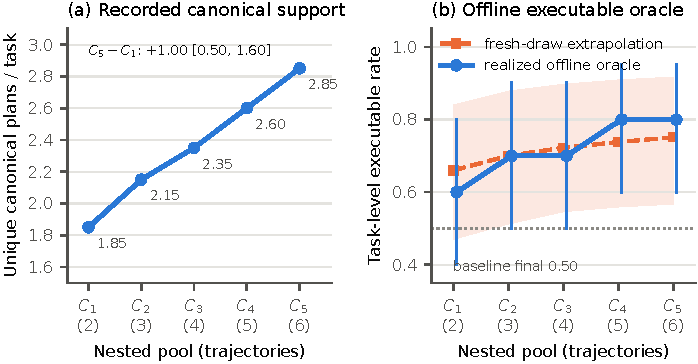
\includegraphics[width=0.78\textwidth]{figures/qwen-candidate-pool-enlargement.pdf}
\caption{Additional independent restarts expand recorded support on 20 Qwen tasks. $C_j$ pools the temperature-zero anchor with $j$ stochastic trajectories (total trajectories in parentheses). (b) Realized offline oracle with 95\% task-bootstrap intervals, and the fresh-draw plug-in extrapolation with its task-cluster band; the dotted line is the temperature-zero final answer, and the aqua line a uniformly random choice among the pool's final answers. Offline oracles are upper bounds, not deployed selector accuracy.}
\label{fig:pool}
\end{figure*}

\subsection{Exploratory mechanism studies}
\label{sec:res-collapse}

Two further studies are exploratory and reported in full in the appendix. A frozen restart-versus-repair gate on eight DeepSeek tasks stopped because only three anchor failures were informative, below the frozen minimum of four, so no main cohort ran (Appendix~\ref{app:repair}). On the two exhausted tasks, sequential temperature-0.7 repairs concentrated on one invalid response (raw modal rates 86.25\% and 95\%). A frozen same-task control kept only the public task and output format, removing the candidate, diagnostic, attempt index, and history together. It also concentrated: TEST0030 returned \texttt{["bookshelf"]} in 79/80 calls (98.75\%), a different mode from its repair-conditioned \texttt{["IMPOSSIBLE"]}, and TEST0535 returned \texttt{["redstone\_torch"]} in 76/80. None of the 160 public-task-only responses was executable. We read this as task-level response collapse on two selected tasks, not a population comparison: raising temperature inside a direct prompt need not diversify a hard failure.

A post hoc held-out planning component control (Appendix~\ref{app:planner}) finds that zero-call symbolic search alone reaches 12/12 feasible PlanCraft replays, versus 8/12 when DeepSeek chooses among verified actions without the symbolic filters (exact $p=0.125$). Because the planner was developed post hoc and its step cap changed after the first held-out batch, we treat it as exploratory evidence that symbolic constraints supply much of the executable support, not as an LLM or multi-agent result.

\subsection{An illustrative fixed-pool selector calculation}
\label{sec:res-selector}

Appendix~\ref{app:selector} gives an illustrative fixed-pool calculation, not a privacy--utility frontier. With binary executor utility on mixed $C_5$ pools ($g_U^{\mathrm{sel}}=\Delta_u=1$), the monotone exponential mechanism selects an executable candidate with mean probability 0.512, 0.575, 0.682, 0.779, and 0.800 at $\varepsilon=0.5,1,2,4,8$, respectively, against a non-private offline oracle of 0.80; under the general calibration the same values require $\varepsilon=1,2,4,8,16$. Only the selected index is covered by the adjacency; candidate texts, prompts, memories, messages, control flow, and the executor are trusted (Appendix~\ref{app:threat}).

\section{Related Work and Implications}

Test-time optimization uses language models as optimizers or textual-gradient generators \citep{yang2023opro,yuksekgonul2024textgrad}. Self-consistency, tree search, and compute-aware inference spend additional test-time computation on diverse samples or structured exploration \citep{wang2022selfconsistency,yao2023tot,zhou2023lats,snell2024testtime}, and repeated sampling raises coverage whenever a verifier can recognize a correct sample \citep{brown2024monkeys}. For agents, \citet{zhu2025ttsagents} study parallel sampling, sequential revision, verifiers, and diversified rollouts. Our nested pools are a narrower realized-support audit inside one runtime, not a new scaling method; the question they add is whether the recorded generator exposed any executable alternative before search or selection is optimized.

Feedback-based agents such as ReAct, Reflexion, Self-Refine, and LATS condition later generation on actions, evaluation, or verbal memory \citep{yao2022react,shinn2023reflexion,madaan2023selfrefine,zhou2023lats}. Multi-agent sampling and layered aggregation seek gains from multiple response sources \citep{li2024moreagents,wang2024moa,xu2026tacomas}, and graph or workflow search optimizes the agent structure itself \citep{zhuge2024gptswarm,hu2025adas,zhang2025aflow}; the audit applies to any of these that select among retained candidates. Self-correction tends to succeed only with reliable external feedback \citep{huang2024selfcorrect,kamoi2024selfcorrection}; our repair gate supplies such feedback and still concentrates on invalid responses on two tasks. Reduced output diversity after preference tuning \citep{kirk2024rlhf} is one candidate explanation that we do not test.

Learned evaluation can track preferences while exhibiting position, self-enhancement, and verbosity biases \citep{zheng2023judge}, and length-controlled evaluation targets the latter confound \citep{dubois2024length}. We instead measure the downstream consequence of an intervention on a score used inside the runtime, rather than a meta-evaluation correlation.

Canary methods test whether rare secrets influence model outputs \citep{carlini2019secret}. Work on indirect prompt injection, memory poisoning, tool-using-agent attacks, and privacy-norm behavior shows that agent state and external observations can carry security- or privacy-relevant information \citep{greshake2023indirect,chen2024agentpoison,debenedetti2024agentdojo,shao2024privacylens}. MEXTRA mounts adaptive black-box extraction against agent memory \citep{wang2025mextra}; our canary audit is a non-adaptive, exact-match check of one runtime's persistent state and complements rather than replaces such attacks (Appendix~\ref{app:closest}).

Differential privacy calibrates randomized releases to sensitivity \citep{dwork2006calibrating,dwork2014foundations}. Report Noisy Max \citep{dwork2014foundations}, the exponential mechanism \citep{mcsherry2007mechanism}, and selection from candidates whose score functions are themselves private \citep{liu2019private} cover distinct private-selection settings. Private prompt optimization \citep{hong2024dpopt} and continual-observation tools \citep{dwork2010continual} protect other bounded channels, but formal privacy does not establish that the protected decision improves task outcomes. An end-to-end private architecture would also need an explicit privacy principal, adjacency, public transcript, and trusted boundary, because memory, messages, stopping time, and topology can leak independently of a private score; routing cross-boundary communication through a privatized summary, billboard style, is one untested route to joint DP \citep{hsu2014private}.

The observed support bottleneck changes the engineering target in this configuration. Better reranking cannot solve generator-unreachable tasks; independent restarts sometimes do, but at three times the token cost. Efficient diversity requires an intervention that changes task-relevant support without multiplying full trajectories, which we leave to future work.

\section{Reproducibility}

Every reported experiment uses a JSON protocol frozen as an internal record before execution, a resumable runner, and machine-readable outputs. The 120-instance persistence replication uses protocol 199, and its complete live and analysis records are archived as artifacts 220 and 222. References are withheld during online generation and exactness is recomputed offline. Repeated calls, trajectories, and candidate slots are clustered by task in uncertainty analyses. Raw canaries and provider credentials are excluded from research artifacts. The appendix records amendments, stopping decisions, and excluded provider-error traces, and Appendix~\ref{app:repro} lists what the anonymous supplement regenerates; the upstream runtime is not redistributed.

\section{Conclusion}

Candidate selection in test-time LLM agents should be preceded by an audit of exposure, score consequences, and realized candidate support. In the audited fixed-topology TacoMAS--PlanCraft configuration, a complete 120-instance canary replication fails to detect post-input exposure and places a 2.5\% one-sided upper bound on the evolve-arm rate under the audited setting. Removing the dominant score term changes recorded scores without a reliably detectable change in exactness, and 43 of 46 failed runs lack a parser-accepted executable candidate, leaving fixed pools only 0 to 8.3 points of headroom. Additional independent restarts raise the offline oracle from 0.60 to 0.80 at triple the token cost. These measurements locate the binding constraint in generation support for this configuration and expose the limits of the present evidence.

\section{Limitations}

Every study disables structural birth/death and edge edits, so the results describe a fixed-topology slice of TacoMAS and do not test topology evolution, structural leakage channels, or selection within evolving workflows. All studies use PlanCraft, and there is no second runtime or benchmark.

The leakage audit covers one synthetic canary family, injected in the round-one query, one model, a five-round horizon, and exact or five-token partial matching. With 0/120 evolve observations it cannot exclude rates below 2.5\% at one-sided 95\% confidence. It does not test semantic paraphrase, encoded or cross-channel reconstruction, task-relevant secrets, adaptive extraction, or provider-side logs, and the positive controls cover the declared channels rather than the round-one injection path. The canary is unrelated to the task, so the audit tests incidental retention. Qwen replicates the score intervention but not leakage.

The length-term removal is paired within task rather than assigned at random, and it changes the whole fast-round signal, so its estimand is a system-level consequence. It does not evaluate whether the separate slow-update Judge LLM improves downstream decisions, and the runtime authors provide no independent justification for the $0.85$ weight.

Headroom depends on the canonical parser and executor. They accept 32\% of candidate slots and agree with reference exactness on all 65 eligible final answers, but rejected slots were not hand-audited, so generation failures may include parser false negatives. The bound covers only recorded candidates and binary target-reaching utility; hidden reasoning, new repairs, and unrecorded tool interactions lie outside it.

The Qwen enlargement study has 20 tasks. Its nested design identifies added-pool gains but not a sign-symmetric treatment test or a same-context, token-matched continuation control. Its plug-in curve assumes conditionally i.i.d.\ restarts beyond the five observed, and costs are provider-recorded token counts. The matched-slot result identifies cross-trajectory coverage in the cached multi-agent runtime, not a causal multi-agent advantage. Beyond a random final-answer baseline, we report no deployed non-private selector.

Several analyses are exploratory or amended after observation: the 42-pair synthesis, the final-inclusive pool amendment (which leaves every value unchanged), the stopped repair gate and its 0.80 threshold, the held-out planner and its 8-to-12 step-cap change, the Qwen gate-token cap, and the exclusion of nine payment-invalid traces. Response collapse is observed on two selected tasks; its prevalence is unidentified. Finally, the study does not provide end-to-end DP: the selector calculation covers only a candidate-validity release under a narrow replacement adjacency and leaves candidate text and the evolving transcript trusted.

\section{Ethical Considerations}

The experiments use a released agent runtime, a public synthetic planning benchmark, and synthetic canaries; they involve no human participants or personal data. The audit is designed to test privacy-relevant persistence without publishing raw canary values or provider credentials. Its failed-to-detect leakage result should not be read as a privacy guarantee for the audited runtime or for LLM agents generally.

\bibliography{references}

\appendix
\sloppy

This appendix preserves protocol and diagnostic details omitted from the eight-page main submission. All quantities derive from the same frozen experimental records underlying the main paper.

\section*{Endpoint status and amendments}

The table below separates outcomes fixed before provider execution from later analytical qualifications. The qualifications preserve the frozen runs and report rather than replace the original records.

\begin{center}
\resizebox{\columnwidth}{!}{%
\scriptsize
\begin{tabular}{>{\raggedright\arraybackslash}p{0.22\columnwidth}>{\raggedright\arraybackslash}p{0.29\columnwidth}>{\raggedright\arraybackslash}p{0.39\columnwidth}}
\toprule
\shortstack{\textbf{Component}} & \shortstack{\textbf{Frozen}\\\textbf{endpoint}} & \shortstack{\textbf{Final status or}\\\textbf{qualification}} \\
\midrule
Canary audit & Post-input exact or five-token partial exposure in the three-arm 120-instance replication & 0/120 in evolve and reset, and 0/120 false positives in no-canary; one-sided 95\% upper bound 2.5\%, reported as failed to detect for the audited setting. \\
Length ablation & Paired exactness and recorded-score differences in each frozen cohort & Cohort results are primary; the 42-pair synthesis was added after cohort inspection and is labeled secondary and outcome-aware. \\
Fixed-pool headroom & Oracle over the recorded candidate surface & Final answers were retained in the support set by an explicit amendment; the pooled cross-cohort summary remains exploratory. \\
Nested trajectory pool & Support and oracle differences for $C_1\subset C_5$ & Nested sign tests were withdrawn because decreases are impossible by construction; task-bootstrap intervals and one-sided bounds were retained. The matched decomposition is slot-matched, not token-matched. \\
Repair gate & Restart versus repair after shared-anchor failure & The stop rule was reached with three informative failures, so no main cohort was run; the result is a stopped diagnostic. \\
Task-level response collapse & Same-task public-only control on the two exhausted tasks & The control was frozen before those calls; the two tasks remain selected mechanism cases, not a population sample. \\
Selector calculation & Closed-form exponential-mechanism probabilities on cached candidates & This is an illustrative narrow-adjacency calculation, not an empirical end-to-end DP experiment. \\
\bottomrule
\end{tabular}%
}
\end{center}

\section{Audit procedure and stop rules}
\label{app:procedure}

The audit is an ordered checklist. Each step has an estimand, a stop rule fixed before the corresponding run, and an escalation rule; the thresholds below are the ones used in this study, not universal defaults.

\begin{enumerate}
  \setlength{\itemsep}{1pt}
  \item \textbf{Exposure.} Estimand: post-input exact or five-token partial canary recovery, evolve versus depth-matched reset. Signal rule (protocol 199): evolve exposure at least 10\%, a positive paired difference, and exact McNemar $p<0.05$ over 120 complete triads. If not met, report a bounded non-detection and do not calibrate privacy for that channel.
  \item \textbf{Score consequence.} Estimand: paired difference in executable or reference exactness when the score term is removed, with a manipulation check on the score itself. The frozen rules check the score scale first and then a utility-improvement criterion; we report a utility interval that contains zero as inconclusive, never as score invalidity. The frozen precise-null rule for the pooled synthesis requires an interval containing zero with upper endpoint below 0.15.
  \item \textbf{Realized support.} Estimand: the hindsight oracle gap $H_i$ over the recorded pool. Rule (protocol 077): fewer than 4/20 recoverable failures stops selector or retention development on that pool.
  \item \textbf{Support expansion.} Only if step 3 stops: enlarge the pool prospectively and re-measure $H_i$ and cost before any private-selection experiment.
\end{enumerate}

Minimum detectable effects follow from the sample sizes: with 120 complete triads, the planning simulation for step 1 gives 94.8\% power for 15\% versus 2\% discordance; with 20 pairs, step 2 needs at least five pure discordances for one-sided exact $p<0.05$ (Appendix~\ref{app:null}). Cost is reported as provider-recorded tokens at every step.

\section{Metric definitions}
\label{app:metrics}

\begin{center}
\resizebox{\columnwidth}{!}{%
\scriptsize
\begin{tabular}{>{\raggedright\arraybackslash}p{0.20\columnwidth}>{\raggedright\arraybackslash}p{0.37\columnwidth}>{\raggedright\arraybackslash}p{0.14\columnwidth}>{\raggedright\arraybackslash}p{0.21\columnwidth}}
\toprule
\textbf{Metric} & \textbf{Definition} & \textbf{Needs reference} & \textbf{Used for} \\
\midrule
Executable validity & Parser-accepted canonical plan that the reference-free executor runs from the initial inventory to the target & No & Headroom, oracles, retention, selector \\
Reference exactness & Canonical final answer equals the reference action list or \texttt{IMPOSSIBLE} label & Yes (offline) & Length-term removal, Table~\ref{tab:audit} \\
Canonical exact & Plan identical to the canonical reference sequence & Yes (offline) & Planner (secondary) \\
Replay validity & Independent environment replay reaches the target & No & Planner, cross-checks \\
\bottomrule
\end{tabular}%
}
\end{center}

On the 65 eligible final answers of Table~\ref{tab:headroom}, executable validity and reference exactness agree in every run. A separate replay of all 48 non-degenerate DeepSeek finals through the public PlanCraft environment reaches the target in exactly the 26 reference-exact rows. Neither check tests parser false negatives on unparseable text.

\section{Threat model and trust boundary}
\label{app:threat}

The two privacy-relevant components answer different questions and use different boundaries.

\begin{center}
\resizebox{\columnwidth}{!}{%
\scriptsize
\begin{tabular}{>{\raggedright\arraybackslash}p{0.20\columnwidth}>{\raggedright\arraybackslash}p{0.36\columnwidth}>{\raggedright\arraybackslash}p{0.36\columnwidth}}
\toprule
& \textbf{Canary audit} & \textbf{Selector calculation} \\
\midrule
Protected unit & A synthetic random canary injected only in the round-one query & One candidate's clipped validity bit (candidate-score replacement adjacency) \\
Observer & Anyone who can read persistent state after the input round: memory, feedback, stored outputs, scores, and slow-update logs & Only the selected index or output \\
Released & Full state snapshots after the input round & The selected index or output \\
Trusted & Runtime code, provider, and extractor & Candidate texts, prompts, memories, messages, control flow, and the executor \\
Out of scope & Adaptive extraction, provider-side logs, structural edits, task-relevant secrets & End-to-end DP of the transcript or of the evolving state \\
\bottomrule
\end{tabular}%
}
\end{center}

A detected canary would show a persistence channel; a non-detection is a bounded failure to detect under this observer, not a guarantee against a stronger one.

\section{Score sources and per-arm consequences}
\label{app:scoreconsequence}

In the 60 initial canary-study runs (15 agent-round scores each), 705 of 900 recorded contribution scores are fast-round heuristic scores and 195 come from slow-update judging. Of the 165 observations scoring at least 0.8, 24 belong to the five successful runs, compared with 75 of 900 observations overall; these observations are clustered within runs. The run-level AUC of the maximum contribution score is 0.755, and the conditional interval in Appendix~\ref{app:bootstrap} resamples instances.

Removing the length term zeroes the length component wherever the fast-round heuristic is computed. The Judge LLM configuration is identical in both arms, but its inputs and the score history passed to the Meta-LLM differ, and recorded calls and tokens differ by arm (Appendices~\ref{app:initiallength} and~\ref{app:qwendetail}). The intervention therefore estimates the consequence of replacing the heuristic for the whole runtime. Both arms run on every task, so arms are paired within task rather than randomly assigned.

\noindent\textit{Endpoint choice.} With final-answer executable validity in place of reference exactness, both non-degenerate cohorts give identical paired differences, intervals, and discordant pairs (DeepSeek 2/0, exact McNemar \(p=0.5\); Qwen 2/3, \(p=1\)). The initial cohort's executable outcomes are not cached (artifact 237).

\section{Reference-firewall calibration failure}

The initial reference-firewall implementation returned online quality zero for all expensive evaluations. The runtime stores a historical best candidate only when quality strictly improves over an initial value of zero. Constant-zero quality could therefore prevent candidate persistence independently of arm assignment. The issue was detected after the first pair and before interpreting its outcomes.

We froze an amendment that marked both cells \texttt{\detokenize{invalid_harness_calibration}}, excluded them from every endpoint and the 3M valid-token cap, retained them in the artifact, and replaced constant zero with the same reference-free text heuristic in both arms. The complete pair was then restarted. The invalid cells used 282,399 tokens; the 20 valid cells used 2,716,894 tokens and 1,083 calls; total observed use was 2,999,293 tokens. This near-miss demonstrates that reference isolation must cover control flow, not merely omit a reference-derived metric from the final table.

\section{Detailed null sensitivity}
\label{app:null}

The initial audit had zero exposure events in 20 evolve instances, with an exact one-sided 95\% upper bound of 13.9\%. The completed replication has zero events in 120 evolve instances, lowering that bound to 2.5\%. Exposure is also zero in the reset and no-canary arms, and each of the three strata has 0/40 evolve exposures. In the paired replication comparison, the observed evolve-minus-reset risk difference is zero and the exact two-sided McNemar test has \(p=1\). These are failed-to-detect results for the audited model, horizon, topology, and canary family, not estimates of a universal exposure rate.

The independent execution-aware validation likewise has low sensitivity. Five pure method-only discordances would be required for one-sided exact \(p<0.05\), an observed risk difference of 0.25 at 20 pairs. Its observed interval [0, 0.15] includes effects that would triple a 5\% base rate.

\section{Development-stage execution-aware retention}
\label{app:retention}

The eight-pair development pilot completed all 16 five-round cells. Execution-aware retention produced one executable-valid and reference-exact final plan; the text heuristic produced none. Both arms had seven malformed final answers. The paired difference was \(1/8=0.125\), with bootstrap interval [0, 0.375], one method-only discordance, and two-sided exact McNemar \(p=1\).

\begin{center}
\resizebox{\columnwidth}{!}{%
\begin{tabular}{lrrr}
\toprule
\textbf{Outcome} & \textbf{Text heuristic} & \textbf{Execution-aware} & \textbf{Difference} \\
\midrule
Executable-valid final answer & 0/8 & 1/8 & +1/8 \\
Reference-trace exact & 0/8 & 1/8 & +1/8 \\
Malformed final answer & 7/8 & 7/8 & 0 \\
Provider calls & 449 & 446 & -3 \\
Recorded tokens & 1,058,730 & 1,018,841 & -39,889 \\
\bottomrule
\end{tabular}%
}
\end{center}

On TEST0080, execution-aware scoring recognized an executable eight-action ladder plan at round 3, assigned it score 1, and retained the same candidate hash. The control assigned its candidate 0.02975 and ended with a sequence beginning with \texttt{\detokenize{bamboo}}, which is not a crafted output and fails at step zero. This demonstrated the intended mechanism in one pair and justified independent validation; it did not establish utility improvement.

\section{Bootstrap handling}
\label{app:bootstrap}

The original X1 run-level AUC is 0.755. In the 100,000-draw instance-cluster bootstrap, 3,903 draws (3.903\%) contain no positive or no negative run and therefore have undefined AUC. The reported [0.651, 0.853] interval is calculated over the 96,097 defined draws and must be read as conditional on resampling both classes. No numerical AUC is imputed for degenerate draws.

For the non-degenerate main cohort, each original-evolve run belongs to a distinct instance cluster. Of 100,000 cluster draws, 51 (0.051\%) are degenerate; the conditional interval over 99,949 defined draws is [0.625, 1.000].

\section{Provider repeatability detail}

Across 20 cache-bypassed temperature-zero calls, two raw response hashes appear. The modal byte-identical rate is 65\%, and pairwise raw-response disagreement is 47.9\%. After parsing and action canonicalization, all 20 outputs are identical and exact. This result is prompt-specific; semantic identity is not implied for other prompts.

\section{Protocol and artifact index}

\begin{itemize}
  \item clustered score correction and null-power analysis: artifacts 063 and 066;
  \item execution-aware development and validation: artifacts 058 and 061;
  \item non-degenerate four-arm replication: artifacts 068 and 069;
  \item arm-level/selector-level notation correction: artifact 100;
  \item Qwen cross-model score replication: artifacts 074 and 075.
  \item Qwen candidate-pool enlargement: protocol 083 and artifacts 084--085.
  \item corrected nested-pool inference and trajectory decomposition: protocol 087 and artifact 088.
  \item public-task-only DeepSeek response-collapse control: protocol 096 and artifacts 097--098.
  \item 120-instance persistence replication: protocol 199, authorization amendment 219, live artifact 220, and complete analysis artifact 222.
\end{itemize}

\section{Implementation clarification}

After the source and intervention audit, the runtime authors clarified the intended role of the contribution signal. The length-based formula is used during regular fast rounds when no slow update is scheduled, as a low-cost and coarse proxy for analytical effort. During a slow update, a separately configured Judge LLM produces an independent score; the Meta-LLM receives that score together with historical heuristic and judge scores and uses them with other state information for topology birth/death, edge edits, feedback, and next-round guidance. The heuristic therefore enters subsequent state and decisions rather than serving only as a log. The authors did not provide an independent validation for the specific $0.85$ length weight. This clarification changes the interpretation of the intervention: it confirms consequential use of the released score while leaving its semantic validity an empirical question.

\section{Initial length intervention}
\label{app:initiallength}

The initial prospective intervention completed ten five-round pairs. Both arms solved TEST0095 and failed the other nine instances. Removing the length term changed mean contribution score from 0.429 to 0.069 and eliminated all 33 score observations at least 0.8, while exactness remained 1/10 in both arms.

\begin{center}
\resizebox{\columnwidth}{!}{%
\begin{tabular}{lrrr}
\toprule
\textbf{Outcome} & \textbf{Original score} & \textbf{Length removed} & \textbf{Paired difference} \\
\midrule
Final executable exact & 1/10 & 1/10 & 0.0 \\
Correctness-regression instances & 0 & 0 & 0 \\
Mean contribution score & 0.429 & 0.069 & -0.360 \\
Contribution scores at least 0.8 & 33 & 0 & -33 \\
Recorded input + output tokens & 1,334,811 & 1,382,083 & +47,272 \\
\bottomrule
\end{tabular}%
}
\end{center}

The paired exactness bootstrap interval [0, 0] is degenerate because no pair is discordant; since $|\mathrm{RD}|$ cannot exceed the discordant-pair rate, the exact two-sided bound on 0/10 discordances gives $|\mathrm{RD}|\le0.31$. The score reduction occurs in all ten pairs. The paired mean difference is -0.360, bootstrap interval [-0.500, -0.225], and exact two-sided sign-test \(p=0.00195\). These statistics validate manipulation of the score scale, not utility improvement.

\section{Independent execution-aware validation table}

\begin{center}
\resizebox{\columnwidth}{!}{%
\begin{tabular}{lrrr}
\toprule
\textbf{Outcome} & \textbf{Text heuristic} & \textbf{Execution-aware} & \textbf{Difference} \\
\midrule
Executable-valid final answer & 0/20 & 1/20 & +1/20 \\
Reference-trace exact & 0/20 & 1/20 & +1/20 \\
Malformed final answer & 14/20 & 14/20 & 0 \\
Provider calls & 1,095 & 1,111 & +16 \\
Recorded tokens & 2,669,935 & 2,604,731 & -65,204 \\
\bottomrule
\end{tabular}%
}
\end{center}

\section{Qwen cross-model replication detail}
\label{app:qwendetail}

The dated \texttt{\detokenize{qwen3.7-max-2026-06-08}} snapshot completes the frozen eight-cell gate and all 40 paired main cells. The initial length-two gate scores 5/8 exact and is selected without fallback-tier search. In the 20-pair main cohort, original and length-zero scoring achieve 11/20 and 10/20 exact, respectively. The paired difference is -0.05 with bootstrap interval [-0.25, 0.15]; two length-zero-only and three original-only successes give one-sided exact \(p=0.8125\).

The causal score endpoint is decisive: the paired mean difference is -0.1167, interval [-0.1503, -0.0837], with lower scores in all 20 pairs. Counts at least 0.8 change from 8/300 to 0/300, paired interval [-0.80, -0.05]. Thus the frozen score-scale rule passes, while the utility rule does not. This is a cross-model replication of the measurement diagnosis, not evidence that length removal improves planning.

The provider's reserved function-name policy requires renaming the read-only PlanCraft \texttt{\detokenize{search}} tool to \texttt{\detokenize{recipe_search}}; its arguments and environment semantics are unchanged in all cells. The runtime tracker reports 4,416,267 tokens and 2,292 calls over 41/48 cells. Seven completed cells have empty usage objects despite full trajectories, so the totals are lower bounds. Credentials are absent from the protocol, artifacts, and raw-output tree.

\section{Qwen intermediate-candidate oracle audit}

Protocol 077 was frozen before candidate-content inspection and makes zero model calls. It evaluates every persisted round-agent answer (three agents by five rounds) and the synthesized final answer from each of the 40 Qwen main cells. Candidate texts are deduplicated by within-run SHA-256; only hashes, locations, lengths, and deterministic diagnostics are retained in artifact 078.

\begin{center}
\resizebox{\columnwidth}{!}{%
\begin{tabular}{lrrrrr}
\toprule
\textbf{Arm} & \textbf{Final executable} & \textbf{Round-candidate oracle} & \textbf{Recoverable failed final} & \textbf{Generation failure} & \textbf{Duplicate slots} \\
\midrule
Original score & 11/20 & 12/20 & 1/20 & 8/20 & 259/320 \\
Length-zero score & 10/20 & 11/20 & 1/20 & 9/20 & 263/320 \\
\bottomrule
\end{tabular}%
}
\end{center}

Both semantic oracle gaps are 0.05 with paired-bootstrap intervals [0, 0.15]. Reference-exact gaps are identical. No finalization failure contains a valid round-5 candidate. The original-score recoverable count is below the frozen 4/20 advancement threshold, so the execution-gated selector route stops without API expenditure. This diagnostic does not prove that generation is the only bottleneck; it shows that selection among the persisted answer candidates has insufficient observed headroom for the planned method.

\section{Cross-cohort headroom and diversity}
\label{app:headroom}

\begin{center}
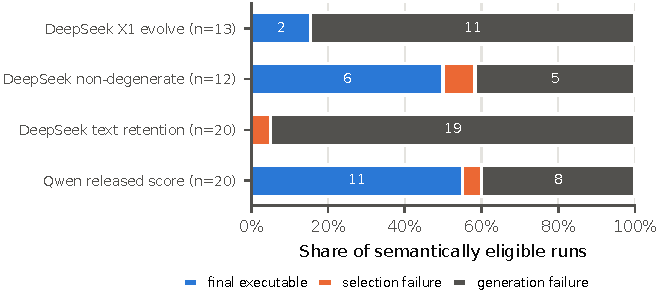
\includegraphics[width=\columnwidth]{figures/failure-decomposition.pdf}
\end{center}
\noindent\textit{Failure decomposition.} In every cohort most failed runs contain no parser-accepted executable candidate in the recorded pool (generation failures); selection failures, where a better selector over the same pool would have succeeded, total three of 46 failures.

\noindent\textit{Estimands and sensitivity.} The round-candidate-only oracle and the final-inclusive oracle are both 22/65, so the amendment below changes no value. Conditional on failure, generation failures are 43/46 (exact 95\% interval [0.821, 0.986]) and selection failures 3/46 ([0.014, 0.179]); as a share of eligible runs, recoverable failures are 3/65 ([0.010, 0.129]). Under reference exactness over all 72 runs, including the seven \texttt{\detokenize{IMPOSSIBLE}} references, the final and pool oracles are 19/72 and 22/72, the same three recoverable runs. Parser acceptance is 43/320 slots for DeepSeek X1 evolve, 95/192 for the non-degenerate arm, 52/320 for text retention, and 175/320 for Qwen (365/1,152 overall). Artifact 231 regenerates these numbers from the cached per-run rows.

\noindent\textit{Parser sensitivity.} The 43 generation failures average 13.6 rejected slots. Were each independently a false negative with probability 1\% (5\%), about 5.4 (21.0) of these runs would hold a valid candidate, so bounding a per-slot rate cannot certify the run count; that requires auditing every unique rejected text in the 46 failed runs (at most 495), which we have not done (artifact 237).


Protocol 080 freezes a zero-call extension to the 60-run DeepSeek X1 cohort, the 48-run non-degenerate main matrix, and the 40-run execution-aware confirmatory cohort. Semantic headroom excludes \texttt{\detokenize{IMPOSSIBLE}} references because forward execution cannot certify non-existence. Diversity and reference-exact summaries retain all runs. The original frozen estimand compared the 15-round-candidate oracle directly with the synthesized final. This comparison is not an upper bound because a synthesizer can in principle create a valid final absent from its input candidates. We retain the original protocol hash and record an outcome-aware amendment that adds the realized final to oracle support. The corrected quantity is weakly nonnegative and bounds selectors that can retain the current final. In the 65 selected semantically eligible original/control runs, the observed frequency of a valid synthesized final with no valid round-agent candidate is 0/65. No model call or run outcome changes.

Across original/control arms, empirical fixed-pool selector headroom is 0/13 for DeepSeek X1 evolve, 1/12 for DeepSeek non-degenerate original evolve, 1/20 for confirmatory text retention, and 1/20 for Qwen original scoring. An outcome-aware exploratory stratified synthesis gives 3/65=0.046, bootstrap interval [0, 0.108]. A two-sided Clopper--Pearson interval is [0.010, 0.129] if the heterogeneous cohorts are treated as exchangeable Bernoulli trials. This is an exact realized-pool bound for selectors restricted to the final plus 15 persisted round-agent candidates; population intervals concern similar-task generalization. Offline headroom in the confirmatory text-retention arm and the prospective execution-aware-minus-control point estimate are both 0.05 on the same 20 tasks, a descriptive convergence rather than an independent mediation test.

Exact-text repetition is provider-specific. Qwen original/length-zero duplicate rates are 0.809/0.822, whereas DeepSeek arms range approximately 0.073--0.272. Canonical parseable-plan support is consistently small: among 72 original/control runs, 38 have zero unique parseable canonical plans, 22 have one, 8 have two, and 4 have at least three. The arms average 0.45--1.05 unique canonical plans per run, and 73\%--91\% of parseable slots duplicate another canonical plan. We therefore distinguish lexical diversity from task-relevant candidate support.

\section{Stratified length synthesis and completeness diagnostic}

The 10-, 12-, and 20-pair length interventions contain 42 pairs. The stratified average exact difference is +0.0238, bootstrap interval [-0.0952, 0.1429], with four length-zero-only and three original-only successes and two-sided exact \(p=1\). This outcome-aware secondary synthesis meets the frozen rule for describing a precise near-zero average: its interval contains zero and its upper endpoint is below 0.15.

The length component's association with well-formed output does not transfer uniformly. DeepSeek original arms yield well-formed-prediction AUCs 0.938 and 1.0, but Qwen yields 0.133 with the opposite mean direction. Paired malformed changes under length removal are 0, -0.167, and +0.15. Thus length may act as a model-dependent formation proxy, but it is not a validated cross-model completeness or semantic-quality signal.

\section{Prospective candidate-pool enlargement}
\label{app:pool}

Protocol 083 was frozen before inspecting any output on 28 untouched reference-length-two PlanCraft tasks. Each task receives one complete uncached temperature-0 trajectory and five independent complete uncached temperature-0.7 trajectories. Thinking is disabled throughout. A trajectory contributes 15 round-agent answers and one synthesized final; canonical plans are deduplicated before support and execution measurement. The nested pool \(C_j\) contains the temperature-0 trajectory and stochastic repetitions 1 through \(j\). This makes \(C_5-C_1\) a randomized generation-budget contrast over an identical task set.

The eight-task gate passes: mean \(S_5-S_1=0.875\), 6/8 tasks have \(S_5\ge2\), all 48 valid trajectories complete five rounds, and all have positive usage. A provider payment interruption had previously created nine persisted traces containing \texttt{Access denied} or \texttt{overdue-payment}; an integrity back-audit marks all nine invalid, including two with partial positive usage. After seven valid tasks, the conservative 6.5M gate-token projection blocked the eighth task because those invalid attempts had consumed budget. The recorded amendment raises only this cap to 7.5M. The original and amended hashes begin \texttt{7ccf128c5bd4} and \texttt{97c35906de54}; the closure manifest stores both complete values. At amendment time, nested nonnegative support gains and the first seven task summaries made both substantive gate conditions mathematically irreversible. No task, condition, endpoint, threshold, or main budget changed.

The 20-task main cohort completes all 120 trajectories without an integrity failure. Results are:

\begin{center}
\resizebox{\columnwidth}{!}{%
\begin{tabular}{lrrrr}
\toprule
\textbf{Contrast} & \textbf{Mean difference} & \textbf{Task-bootstrap 95\% interval} & \textbf{One-sided 95\% lower bound} & \textbf{Exact test} \\
\midrule
Canonical support, \(C_5-C_1\) & +1.00 & [0.50, 1.60] & 0.60 & withdrawn: nested \\
Executable oracle, \(C_5-C_1\) & +0.20 & [0.05, 0.40] & 0.05 & withdrawn: nested \\
Headroom over baseline final, \(C_5-C_1\) & +0.20 & [0.05, 0.40] & 0.05 & withdrawn: nested \\
Standalone support, temperature 0.7 minus 0 & -0.05 & [-0.35, 0.25] & not applicable & \(p=1.0\) \\
\bottomrule
\end{tabular}%
}
\end{center}

The nested support/oracle/headroom curves are 1.85/0.60/0.10, 2.15/0.70/0.20, 2.35/0.70/0.20, 2.60/0.80/0.30, and 2.85/0.80/0.30 for \(C_1\) through \(C_5\). The originally reported nested sign-test values are invalid because decreases are excluded by construction and are formally withdrawn in artifact 088. The non-nested standalone temperature contrast permits either direction and retains its \(p=1\) result.

The trajectory decomposition contains 57 successful stochastic trajectories among 100. The anchor-inclusive plug-in oracle estimates are 0.660, 0.700, 0.722, 0.738, 0.751, 0.784, and 0.798 for \(n=1,2,3,4,5,10,\) and \(20\). The \(n>5\) values assume conditionally i.i.d. trajectories and are extrapolations. Task-cluster intervals, rather than trajectory-level independent intervals, preserve the 20-task experimental unit.

Per task, the nested oracle pattern from \(C_1\) to \(C_5\) is all-success for 12 tasks, all-failure for four, rescued at \(C_2\) for two, and rescued at \(C_4\) for two. Support gains \(C_5-C_1\) are 0 for eight tasks, 1 for eight, 2 for two, 3 for one, and 5 for one. Task-bootstrap intervals for the realized oracle are [0.40, 0.80] at \(C_1\), [0.50, 0.90] at \(C_2\) and \(C_3\), and [0.60, 0.95] at \(C_4\) and \(C_5\). Of the four \(C_5\)-only rescues, TEST0102, TEST0105, and TEST0361 contain a valid plan in 1/5 stochastic trajectories; TEST0526 contains one in 4/5. Five stochastic final answers alone attain 0.65 oracle coverage. A uniformly random final answer of \(C_j\) is executable 0.50, 0.52, 0.53, 0.55, and 0.54 of the time; the oracle's lead grows from 0.10 [0, 0.23] to 0.26 [0.10, 0.43]. A random stochastic slot is executable about 0.41 of the time. Score-based selectors cannot be replayed from the cached per-trajectory counts. At a matched count of 16 slots, cached cross-trajectory mixing has expected oracle 0.626 versus 0.570 within one stochastic trajectory, difference 0.056, task-bootstrap interval [0.016, 0.105]. All trajectories use the same three-agent runtime, so this is not a single-agent comparison.

Main-cohort generation costs are 4,807,489 recorded tokens for \(C_1\) and 14,430,644 for \(C_5\). The incremental four trajectories consume 9,623,155 tokens, a total ratio of 3.0017. Across gate and main, 168 valid trajectories record 10,546 calls and 20,489,906 tokens. Including the nine retained integrity-failed attempts gives 10,590 calls and 20,573,345 recorded tokens.

For cached \(C_5\) candidates, binary valid-versus-invalid executor utility gives \(g_U^{\mathrm{sel}}=\Delta_u=1\) and hence local \(\rho_U^{\mathrm{sel}}=1\) whenever a mixed-validity pool exists. This candidate-level ratio is distinct from the arm-level ablation consequence \(\delta_V^{\mathrm{abl}}\). The earlier artifact 071 conflated these estimands and its epsilon inversion is withdrawn; artifact 100 records the zero-call correction. The monotone exponential mechanism gives mean exact valid-selection probabilities 0.5119, 0.5748, 0.6822, 0.7793, and 0.7996 at \(\varepsilon=0.5, 1, 2, 4,\) and \(8\). These values are the expected consequence of a maximally separated binary signal on a small pool, not an independently discovered frontier. Under candidate-score replacement adjacency, one candidate's clipped validity bit may change and only the selected index/output is released; candidate text and the remaining system are trusted.

\section{Stopped DeepSeek compute-matched generation gate}
\label{app:repair}

Protocol 090 freezes a non-nested restart-versus-repair comparison before any provider call on 20 untouched reference-length-two tasks: eight adaptive gate candidates and 12 reserved main tasks. Each task receives a shared temperature-0 five-round, three-agent trajectory. An executable anchor-pool candidate causes symmetric success and zero added intervention calls. On anchor failure, a new temperature-0.7 trajectory defines realized token cap \(B_i\); sequential direct repair candidates count toward the primary pool only while cumulative repair tokens do not exceed \(B_i\). Repair uses the public task and reference-free executor diagnostic, never the hidden reference. Unsuccessful repair stops at its first budget crossing or 80 calls.

All eight gate tasks complete with provider integrity. Five anchors succeed, so only TEST0181, TEST0030, and TEST0535 are informative. Their outcomes are:

\begin{center}
\resizebox{\columnwidth}{!}{%
\begin{tabular}{lrrrrr}
\toprule
\textbf{Task} & \textbf{Restart} & \textbf{Repair} & \textbf{Restart tokens} & \textbf{Included repair tokens} & \textbf{Repair calls} \\
\midrule
TEST0181 & 0 & 1 & 157,910 & 1,008 & 1 \\
TEST0030 & 0 & 0 & 138,559 & 51,330 & 80 \\
TEST0535 & 0 & 0 & 162,193 & 50,313 & 80 \\
\bottomrule
\end{tabular}%
}
\end{center}

The frozen gate requires at least four informative anchor failures. It therefore stops even though repair has at least one rescue, does not underperform restart in rescue count, all provider records pass integrity, and both failed repair branches reach the 80-call exhaustion rule. No main task is run. Conditional on anchor failure, repair minus restart is +0.333 with task-bootstrap interval [0, 1] and exact paired \(p=1\). We do not interpret an all-eight difference because five symmetric successes are inherited from the shared anchor rather than caused by either intervention.

Repair diversity is the principal diagnostic. TEST0181 succeeds immediately with \texttt{\detokenize{["dark_oak_planks", "pink_bed"]}}; because it stops after one call, its modal concentration is not estimable. TEST0030 has only three raw response forms over 80 calls: 69 \texttt{\detokenize{["IMPOSSIBLE"]}}, nine \texttt{\detokenize{IMPOSSIBLE}}, and two empty responses. Its raw modal rate is 86.25\%, semantic normalization combines the first two forms into an \texttt{\detokenize{IMPOSSIBLE}} intent in 78/80 calls (97.5\%), and semantic pairwise agreement is 95.1\%. TEST0535 also has three raw forms, with \texttt{\detokenize{["redstone_torch"]}} appearing 76/80 times (95\% raw and semantic modal rates; 90.4\% semantic pairwise agreement); the missing intermediate \texttt{\detokenize{redstone}} makes it non-executable. Across the two exhausted tasks, the call-weighted raw modal share is 145/160=90.625\%, and the semantic share is 154/160=96.25\%.

The repair-only 0.80 threshold was introduced after observing the stopped gate and was not part of a frozen protocol. Calls within a task are not independent task units: the observed 86.25\%--95\% raw range comes from two failures only. Failure-type association is not estimable with three repair branches, and cross-cohort modal stability is unavailable because earlier disjoint DeepSeek cohorts did not record repeated direct repairs under this prompt. The executor behaves as intended in both failures: it does not certify \texttt{\detokenize{IMPOSSIBLE}}, and it rejects plans that omit required intermediate products.

We then froze protocol 096 before making a same-task public-only control. Each exhausted task received 80 additional DeepSeek temperature-0.7 calls with the same output-format instruction but no candidate, executor diagnostic, attempt index, response history, or reference. TEST0030 produced raw \texttt{\detokenize{["bookshelf"]}} in 79/80 calls (98.75\%), a different invalid mode from its repair-conditioned \texttt{\detokenize{["IMPOSSIBLE"]}}; TEST0535 produced raw \texttt{\detokenize{["redstone_torch"]}} in 76/80 and the same semantic plan in 80/80. No response was executable. Both tasks exceed the 0.80 near-determinism threshold frozen in protocol 096, and the mean task-level conditioned-minus-public-only raw modal-rate contrast is -0.0625. The control removes the candidate, diagnostic, attempt index, and history together, so it is not a single-factor intervention; it does not support conditioning as the cause. We use \textbf{task-level response collapse} for the repeated invalid endpoint under both direct prompts. Protocol 096 treats the two tasks as the independent units and forbids a call-level population test.

The first two direct calls on TEST0030 reached the output limit in hidden reasoning and exposed empty visible answers because the direct path omitted the full runtime's explicit non-thinking switch. Both calls, 3,768 tokens, and malformed outcomes remain in the intention-to-repair record; excluding them, TEST0030's raw modal rate is 69/78 (88.5\%) and its semantic modal rate 78/78. Subsequent direct calls pass \texttt{\detokenize{thinking.type=disabled}}; no prior output is deleted or rerun. LiteLLM response caching is disabled throughout, while DeepSeek's automatic provider-side prefix-cache accounting is separately outside that client flag. Total gate usage is 736 calls and 1,642,567 recorded tokens: 1,081,254 anchor, 458,662 restart, and 102,651 repair tokens. TEST0181 shows only that repair succeeded on its first attempt while a matched-budget restart failed; comparing first-draw tokens with a fully spent failed trajectory as a multiplicative efficiency ratio would be misleading. This stopped gate is positive mechanism evidence about two observed failures, but not a positive comparative-method claim.

\section{Held-out planning component control}
\label{app:planner}

The planner was developed post hoc on nine earlier PlanCraft screening tasks: DeepSeek selects one verifier-applicable recipe output per step, options are restricted to those with minimum finite post-action distance to the target, and a bounded symbolic pre-check (depth 12, 50,000 states) emits \texttt{IMPOSSIBLE} only when it exhausts its state space without a target. Its first held-out batch of nine tasks used an eight-step cap and truncated the three long tasks; the cap was then raised to 12 and the same batch rerun, after which a second batch of nine ran unchanged. Bounded stops are not global impossibility proofs. Reported separately: on the nine development tasks the final planner reached 7/7 feasible targets; the first held-out batch reached 3/6 feasible targets at the eight-step cap and 6/6 after the cap change; the untouched second batch reached 6/6 feasible targets with 4/6 canonical exact and 3/3 bounded stops. Only the second batch is a clean held-out evaluation. The final planning diagnostic used this frozen 18-task cohort and no new benchmark selection. The symbolic-only control reproduces 12/12 feasible replays, 8/12 canonical exact plans, six bounded stops on impossible-reference tasks, and 14/18 evaluator-exact labels. Ten of the 12 feasible cached plans are sequence-identical to the symbolic plans; the two remaining replay-valid plans use alternative action orderings. Only 7/78 accepted requests exposed multiple options, and four step-index mismatches occurred in two replay-valid tasks. These branch-level quantities are descriptive for the fixed cohort.

The prospective unfiltered DeepSeek arm removes bounded pre-checks and distance filtering but retains local action verification. It uses 142 provider calls and 43,623 recorded tokens, reaching 8/12 feasible targets with 5/12 canonical exact plans. Against symbolic search, replay has four symbolic-only and no live-only pairs (two-sided exact $p=0.125$); canonical matching has four symbolic-only and one live-only pair ($p=0.375$). The six impossible-reference runs terminate without reaching a target, which does not certify impossibility. This component comparison is separate from architecture-level inference and is not a causal multi-agent result.

\section{Closest work}
\label{app:closest}

\begin{center}
\resizebox{\columnwidth}{!}{%
\scriptsize
\begin{tabular}{lccccc}
\toprule
\textbf{Work} & \textbf{Adaptive extraction} & \textbf{Persistent state} & \textbf{Support bound} & \textbf{Private selector} & \textbf{Benchmark} \\
\midrule
MEXTRA \citep{wang2025mextra} & Yes & Agent memory & No & No & Memory-based agents \\
Agent TTS \citep{zhu2025ttsagents} & No & No & Partial & No & Agent benchmarks \\
This paper & No & Fixed-runtime state & Yes & Calculation only & PlanCraft \\
\bottomrule
\end{tabular}%
}
\end{center}

\section{Fixed-pool selector calculation}
\label{app:selector}

\noindent\textit{Setting.} The candidate set of a pool, its size $k$, and the output domain (the $k$ indices) are fixed and public. Each candidate $j$ has a clipped score $u_j\in[0,\Delta_u]$; here $u_j$ is binary executor validity and $\Delta_u=1$. Two inputs are neighbors under candidate-score replacement adjacency if they differ in the score of one candidate $i$ by at most $\Delta_u$. Candidate texts and everything else are trusted and unreleased.

\noindent\textit{Claim.} The mechanism $M$ that outputs $j$ with probability $w_j/Z$, where $w_j=\exp(\varepsilon u_j/\Delta_u)$ and $Z=\sum_l w_l$, is $\varepsilon$-DP under this adjacency.

\noindent\textit{Proof.} Let a neighbor raise $u_i$ by $\delta\in[0,\Delta_u]$, giving weights $w'$ and normalizer $Z'=Z+w_i(e^{\varepsilon\delta/\Delta_u}-1)$, so $Z\le Z'\le e^{\varepsilon\delta/\Delta_u}Z$. For $j=i$: $\Pr[M'=i]/\Pr[M=i]=e^{\varepsilon\delta/\Delta_u}Z/Z'\le e^{\varepsilon}$, and the reverse ratio is $e^{-\varepsilon\delta/\Delta_u}Z'/Z\le1$. For $j\ne i$: $\Pr[M'=j]/\Pr[M=j]=Z/Z'\le1$ and the reverse ratio is $Z'/Z\le e^{\varepsilon}$. A decrease is symmetric. This is the monotone case of the exponential mechanism \citep{mcsherry2007mechanism}; under adjacencies where several scores can move in opposite directions, the general calibration $\exp(\varepsilon u_j/2\Delta_u)$ is required, which doubles every budget.

\begin{center}
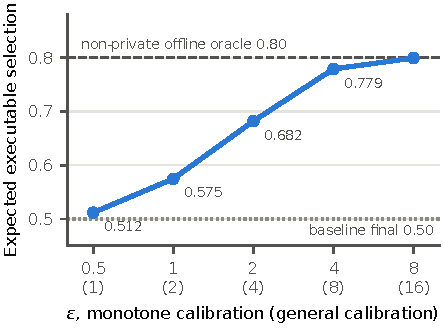
\includegraphics[width=0.85\columnwidth]{figures/selector-calculation.pdf}
\end{center}
\noindent\textit{Values.} Means over the 20 cached $C_5$ pools (pools without a valid candidate contribute 0, so the ceiling is the 0.80 offline oracle). Labels give $\varepsilon$ under the monotone calibration with the general-calibration equivalent in parentheses. This is not a deployed selector, not a privacy--utility frontier, and not end-to-end privacy.

\section{Reproducibility supplement}
\label{app:repro}

The anonymous supplement contains the frozen protocols released with this paper, the cached analyses 037, 080, 081, 087, and 088, the replication summary 223, and our analysis, reanalysis, and figure scripts. Running the reanalysis script regenerates the counts in Table~\ref{tab:headroom}, the generation- and selection-failure counts and intervals, the parser acceptance rates, the per-task pool patterns and intervals of Figure~\ref{fig:pool}, the score-source counts of Figure~\ref{fig:audit}c, and the canary denominators; artifact 237 adds the random-final baselines, endpoint comparison, and parser sensitivity; the figure script redraws Figures~\ref{fig:audit} and~\ref{fig:pool} and the appendix figures. The upstream TacoMAS runtime is not redistributed because its license could not be confirmed, so live runs require a separate checkout. Models are DeepSeek V4 Flash and the dated \texttt{\detokenize{qwen3.7-max-2026-06-08}} snapshot, with thinking disabled, client-side response caching disabled, temperature 0 for anchors and audits, and temperature 0.7 for stochastic trajectories, repairs, and public-only calls. The PlanCraft task file used by the replication has SHA-256 prefix \texttt{1d41af11279c}.



\end{document}
